
\documentclass[12pt, a4paper, english, brazil]{article}

% Sistema autor-data com títulos nas referências em negrito
% \usepackage[alf,abnt-emphasize=bf]{abntex2cite}

% \usepackage[alf,abnt-emphasize=bf,abnt-repeated-author-omit=yes,abnt-year-extra-label=yes]{abntex2cite}	% Citações padrão ABNT

% ----------------- link in the PDF
% http://tug.ctan.org/macros/latex/contrib/abntex2/doc/abntex2cite.pdf
%Usando o pacote abntex2cite autonomamente ... é preciso passar a opção carregando o pacote url antes do abntex2cite
\usepackage[hyphens]{url}
\usepackage[bookmarks=false]{hyperref}
\usepackage{hyperref}
% ----------------- link in the PDF

\usepackage[alf,abnt-emphasize=bf,abnt-repeated-author-omit=yes]{abntex2cite}

\usepackage[utf8]{inputenc}	
\usepackage[brazil]{babel}
\usepackage{graphicx,url}
\usepackage{subfigure}
\usepackage{enumitem}
\usepackage{amsfonts}
\usepackage{amsmath}

\usepackage{physics}
\usepackage{comment}

\usepackage{lscape}

\usepackage{fancyhdr}

% -
\usepackage{indentfirst}
% \graphicspath{{img/}}
%\pagestyle{empty}

\usepackage{xcolor}

\newcommand{\textRed}[1]{{{\color{red} #1}}}
\newcommand{\textBlue}[1]{{{\color{blue} #1}}}
\newcommand{\dotsBlue}{\colorbox{orange}{\textcolor{blue}{\dots}}}
\newcommand{\boxRed}[1]{\colorbox{red}{#1}}
\newcommand{\boxYellow}[1]{\colorbox{yellow}{#1}}
\newcommand{\linePage}{--------------------------------------------------------------------------------------------------------------}

\usepackage{tabularx}
\newcolumntype{L}{>{\raggedright\arraybackslash}X}
% -

\textwidth 16cm \textheight 23.2cm
\voffset -1.5cm \hoffset -1.4cm

\sloppy

\begin{document}

\rhead{\thepage}
\pagenumbering{arabic}

\begin{center}
	\bf{\LARGE{PROJETO DE DISSERTAÇÃO}\\ $\ $\\}
	\Large{Programa de Mestrado em Ciência da Computação\\
		Universidade Federal de Uberlândia}\\ $\ $\\
\end{center}

\begin{center}
	\bf{Aluno: João Batista Ribeiro\\ $\ $\\
		Orientador: Prof. Dr. André Ricardo Backes\\ $\ $\\
		Coorientador: Prof. Dr. Maurício Cunha Escarpinati\\ $\ $\\
		Data da formalização da coorientação no colegiado: \colorbox{yellow}{xx/xx/2021}\\ $\ $\\
		Título do Trabalho: \colorbox{yellow}{Detecção de linhas de plantio em plantações de cana-de-açúcar}\\ $\ $\\
		Data de Início como Aluno Regular: março de 2021\\ $\ $\\
		Previsão da Defesa: fevereiro de 2023\\ $\ $\\}
\end{center}

\textRed{Versão 0.1 - 22/09/2021}

\section{Introdução}

O rápido crescimento populacional, principalmente do último século, tem impulsionado a demanda por alimentos e a utilização inteligente/sustentável dos recursos naturais. Nesse contexto agricultura aliada tecnologia, chamada de Agricultura de Precisão (AP), busca suprir essa demanda utilizando os recursos sob medida com base nas informações fornecidas pela tecnologia. A AP engloba técnicas de análise espacial da área plantada, informações do solo e das plantas, permitindo aos produtores planejar e monitorar suas plantações \cite{Blasch_2020}.

A Agricultura de Precisão se tornou possível graças ao desenvolvimento e avanços de diferentes tecnologias, como o Sistema de Posicionamento Global (GPS), imagens de satélites, Processamento Digital de Imagens (PDI) e Visão Computacional, sensoriamento remoto entre outras. Possibilitando o desenvolvimento de metologias/técnicas/ferramentas/programas que são aplicados nas várias etapas da agricultura, desde análise e preparação do solo (escassez de determinado nutriente em certa região) até utilização de veículos autônomos para fazer a pulverização de defensivos (com quantidade específica para cada parte do talhão) e na colheita seguindo as linhas de plantio. Muitos dos avanços na AP são fortemente dependentes das tecnologias de processamento digital de imagens \cite{Bolfe_2020}.

As imagens utilizadas na AP têm variadas fontes (e.g., câmeras acopladas em Veículos Aéreos Não Tripulados (VANTs) e satélites) dependendo da aplicação e do \textit{Ground Sample Distance} (GSD) requisitado. GSD refere-se à distância da amostra ao solo, ou seja, quanto cada pixel da imagem obtida representa da região fotografada. Assim quanto menor for o GSD, mais detalhes a imagem terá da região analisada. Satélites (com GSD em média de metros) conseguem imagem de grande regiões mais facilmente que os VANTs (GSD em média de centímetros), que necessitam de planos de voo para abranger toda região e mosaicagem para combinar as imagens obtidas \cite{Messina_2020}.

As imagens de satélites podem ter custo baixo até elevado (dependendo da qualidade das imagens), mas com baixa temporalidade (imagens de uma mesma área em momentos diferentes), baixo nível de detalhes (maior GSD) em relação aos VANTs e sofrem bastante com as condições climáticas (e.g., nuvens). Por outro lado os VANTs, geralmente têm custo baixo para aquisição das imagens, possibilitam a captura (e recaptura) das imagens assim que necessário (alta temporalidade e disponibilidade), com grande nível de detalhes (pequeno GSD) e não sofrem muito com as nuvens devido a altitude de voo \cite{Candiago_2015, Delavarpour_2021}.

Uma das aplicações importantes da AP é a detecção das linhas de plantio, principalmente porque é utilizada como uma etapa importante para outras aplicações da AP (e.g., detecção de ervas daninhas, mapeamento e previsão de produção de safra, detecção de falhas), além de ser usada pelos veículos autônomos \cite{Hassanein_2019}.

A detecção de linhas de plantio é uma tarefa complexa e com vários desafios. Por exemplo, presença de ervas daninhas com assinatura espectral e cor semelhantes a linhas da cultura. Crescimento irregular da cultura, falhas no plantio, imperfeições e oclusões linha de plantio, manchas solo e tipos diferentes na mesma plantação, presença de artefatos bloqueando a visão de linha de cultivo (e.g., árvores), sombras, além de variações nas condições climáticas e de iluminação \cite{Rabab_2021, Doha_2021}.

Um dos cenários de grande utilização da Agricultura de precisão no Brasil é no cultivo de cana-de-açúcar (\textit{Saccharum officinarum}), motivando pesquisadores (e.g., \citeonline{Souza_2017, Souza_2018, Silva_Escarpinati_Backes_2021}) e empresas (e.g., \citeonline{AERO_2017, Sensix_2020, Inforow_2021}) a desenvolverem soluções na área.

O Brasil é o maior produtor e exportador de cana-de-açúcar, com aproximadamente 10 milhões de hectares de área plantada, sendo que mundialmente esse valor é de um pouco mais de 26 milhões de hectares \cite{Ritchie_2020, IBGE_2021, FAOSTAT_2021}. O seu cultivo é de grande importância para a economia brasileira devido as suas diversas aplicações. A cana-de-açúcar pode, por exemplo, ser consumida fresca na alimentação humana e forragem na alimentação animal, produção de açúcar, bebidas, energia e combustíveis, além dos seus subprodutos como o bagaço e a palha podem ser utilizados na fertilização do solo \cite{Oliveira_2018}.

A cana-de-açúcar é uma cultura semi-perene (seu manejo pode durar anos sem ser necessário um novo plantio), o que adiciona uma motivação a mais para detectar as suas linhas de plantio em relação a outras culturas (e.g., milho). Após a primeira colheira, a rebrota da soqueiras pode colhida anualmente por cerca de 5 a 7 anos ou mais \cite{Rudorff_2010}. Contudo também adiciona um desafio, dependendo do estágio da plantação, folhas secas estão presentes no solo entre as linhas da cultura, dificultando a análise computacional \cite{Silva_2020}.

Apesar de na literatura já existir muitos trabalhos para detectar linhas de plantio, a maioria deles são para outras culturas (e.g., milho e beterraba) e com imagens de muito baixas altitudes ($< 2$ m), tiradas a partir do solo (manualmente ou acopladas maquinário agrícola) ou de alta altitudes (imagens de satélites).

Outro ponto importante, não foi encontrado nenhum \textit{software} gratuito e de código aberto que faça detecção das linhas de plantio suficiente bem (em cana-de-açúcar ou outra tipo de cultura), apenas \textit{softwares} comerciais. Assim este projeto também busca desenvolver uma metodologia de detecção das linhas de plantio que possa ser utilizada no desenvolvimento de um \textit{software}, promovendo uma democratização do conhecimento.

\textRed{Adicionar um parágrafo comentando os principais trabalhos de modo bem resumido?}
Na literatura, o trabalho de \citeonline{Silva_2020} contribuiu significativamente para detecção das linhas de plantio em plantações de cana-de-açúcar, contudo não obteve bons resultados com linhas curvas (gerando um efeito serrilhamento indesejado). \textRed{Na abordagem com redes neurais \dotsBlue}.

Considerando o cenário de grande utilização dos VANTs para obtenção de imagens para a Agricultura de precisão, a grande importância da detecção das linhas de plantio, este projeto tem como foco a detecção de linhas de plantio de cana-de-açúcar (uma dos principais cultivos do Brasil, fortemente depende detecção das linhas de plantio para o replantio - correção de falhas, estimativa de produção, qualidade da vegetação entre outros).

%\subsection{Motivação}
    % Deixar dentro da introdução
 
\subsection{Objetivos e Desafios da Pesquisa}
    % => Descreva claramente os desafios que o tema propõe e quais os objetivos que se pretende alcançar. Se o tema for muito abrangente, descreva os objetivos em termos de ``objetivo geral'' e ``objetivos específicos''. Cuidado com objetivos como ``desenvolver um sistema...''; ``explorar um método...'' Esses objetivos são triviais, ou seja, uma vez desenvolvido o sistema ou explorado o método, independente dos resultados, o objetivo foi atingido. Prefira verbos como: ``contribuir'', ``analisar'', ``investigar'', ``comparar''. Os membros da banca ao lerem essa seção farão o seguinte questionamento: Algum conhecimento novo para a humanidade foi produzido?

Este projeto tem como objetivo analisar os métodos de segmentação automática em imagens de VANTs tendo, inicialmente, foco em imagem de plantio de cana-de-açúcar e propor melhorias na detecção de linhas de plantio. 

$=>$ \textRed{talvez} Inicialmente apenas imagem RGB, ou seja, com as 3 bandas, talvez pode ser interessante depois imagem com a banda infravermelho ou infravermelho próximo (dependendo da disponibilidade)

Este projeto tem como objetivos específicos:
\begin{itemize}
    \item Estudar e analisar os métodos propostos na literatura correlata para detecção das linhas de plantio, como por exemplo, transformada de Hough e Radon, segmentação, redes neurais convolucionais, índices de vegetação, operações morfológicas.

    \item Avaliar a detecção de linhas de plantio utilizando as imagens de VANTs em métodos de \textit{Deep Learning} com Índice de Vegetação. Vale mais a pena usar apenas as imagens brutas para treinar uma rede neural ou fazer um pré-processamento e utilizar como entradas a imagem e variados Índices de Vegetação?

    \item Propor melhorias na detecção das linhas de plantio (com linhas retas e curvas) de imagens obtidas por VANTs nas plantações de cana-de-açúcar com plantas em variados estágios (antes do primeiro corte (cana-planta) e depois do primeiro corte (cana-soca)).

    \item \textRed{Colocar também a parte de detecção das falhas no plantio?}
    
    \item Aplicar a proposta em imagem reais de plantações de cana-de-açúcar, analisar e avaliar os resultados provenientes das melhorias com ajuda de especialistas.

    \item \textRed{talvez} Avaliar o método proposto em outros tipos de cultura, como milho, café e algodão.
\end{itemize}

% \subsection{Hipótese} 
    % => Descreva claramente quais são as hipóteses da sua pesquisa (Uma hipótese é uma suposição para a solução do problema que você pretende desenvolver). Indique quais perguntas estão associadas a sua hipótese. Lembre-se que as hipóteses deverão ser comprovadas via os experimentos propostos na seção que descreve o método de pesquisa.
% => colocar nos objetivos

\subsection{Contribuições}
    % => Liste as contribuições do seu trabalho. 
    \textRed{O que colocar em contribuições?}

\section{Revisão da literatura correlata}
    % => Descreva os principais trabalhos existentes na literatura da área que estão relacionados com o trabalho que você está propondo e deixe claro qual a sua contribuição em relação a estes trabalhos. O que você está propondo de novo que estes trabalhos não abordaram ou abordaram de forma ineficiente? Eventualmente, se for o caso, introduza nesta seção os conceitos teóricos existentes na literatura que são necessários para a descrição de seu projeto de tese.

Esta seção apresentará os principais conceitos utilizados neste projeto, bem como alguns trabalhos relacionados.

\subsection{Processamento Digital de Imagens}

\textRed{mudar o título par Pré-processamento?}

O Processamento Digital de Imagens (PDI) compreende a manipulação de imagens digitais por um computador de modo a atingir um objetivo específico com procedimentos envolvendo varias etapas. 

O pré-processamento é uma dessas importantes etapas, onde são feitos ajustes na intensidade dos pixels (sem conhecimento sobre o que representam). Esses ajustes visam remover imperfeições (e.g., presença de pixels ruidosos, contraste e/ou brilho inadequado) geradas no processo aquisição das imagens e realçar detalhes importantes para análise. Assim tem como objetivo melhorar a imagem original para ser utilizada no processamento principal \cite{Marques_Filho_1999}.

Dependendo do contexto da aplicação muitas as técnicas de pré-processamento podem ser utilizadas, dentre elas a correção de brilho e contraste, realce de brilho, realce de bordas. Neste projeto serão utilizadas para preparar as imagens para etapa de segmentação e destacar as linhas de plantio.

\subsubsection{Segmentação}
A segmentação de imagens tem como objetivo dividir a imagem em regiões ou objetos de interesse. O nível de divisões depende do problema a ser resolvido e processo deve ser parado somente após detectar todos objetos de interesse. A segmentação de imagens é considerada umas das tarefas mais difíceis do PDI, já que implica diretamente no resultado da etapa de análise. Assim é importante analisar bem qual técnica de segmentação utilizar para aumentar a probabilidade de se obter uma segmentação precisa \cite{Gonzalez_Woods_2010}.

Ao fim da etapa de segmentação a imagem está divididas em várias regiões e sem sobreposição entre elas, ou seja, cada pixel pertence somente a uma região de interesse. \dotsBlue

\subsubsection{Limiarização}
A Limiarização (\textit{Thresholding}, em inglês) consiste na divisão da imagem em duas classes (fundo e objeto) a partir de um limiar $T$. Caso o valor do pixel for maior ou igual a $T$ terá valor 1 na imagem gerada, caso contrário recebe valor 0. Como resultado produzirá uma imagem binária (com pixels de valor 0 ou 1), processo também chamado de binarização \cite{Kuruvilla_2016}.

A escolha do limiar é uma tarefa complicada e pode não conseguir separar bem as duas classes. Deste modo um limiar local, utilizando pequenas regiões da imagem pode ter melhor resultado. Outra abordagem é a utilização múltiplos limiares, onde a imagem é divida em função dos intervalos dos limiares \cite{Gonzalez_Woods_2010}.

O limiar pode ser escolhido manualmente ou através de algoritmos. Para escolha desse limiar muitos trabalhos na área de segmentação das linhas de plantio utilizam o método de Otsu. Este método \cite{Otsu_1979} utiliza histograma da imagem e busca um limiar ideal que separe a imagem em duas classes (objeto e fundo), de modo maximizar a variância entre as classes e minimizar a variância interna das classes.

\subsubsection{Transformada de Radon}

\subsubsection{Transformada de Hough}

\subsubsection{Operações Morfológicas}

\subsubsection{Índices de vegetação}

\subsection{Deep Learning}

\subsection{Trabalhos relacionados}

\cite{Souza_2017} \dotsBlue

\linePage

\cite{Souza_2018} \dotsBlue

\linePage

Em \citeonline{Silva_2020} foi desenvolvido duas abordagens para detecção de linhas de plantio de cana-de-açúcar, a primeira utilizando algoritmo genético resultando em \citeonline{Silva_Escarpinati_Backes_2021} e a segunda utilizando redes neurais artificiais. Na primeira abordagem também foi utilizado método de Otsu e transformada de Radon (\autoref{fig:2021_silva_flow_chart}). Para comparar os resultados obtidos foram utilizados 4 \textit{datasets} e suas respectivas linhas de plantio marcadas por um especialista. Os \textit{datasets} utilizados têm canas-de-açúcar em variados estágios (idades). As marcação do especialista foram feitas onde existe a linha de plantio e também onde deveria existir, ou seja, locais de falhas no plantio também foram marcados como linha de plantio.

\begin{figure}[htbp]
    \centering
    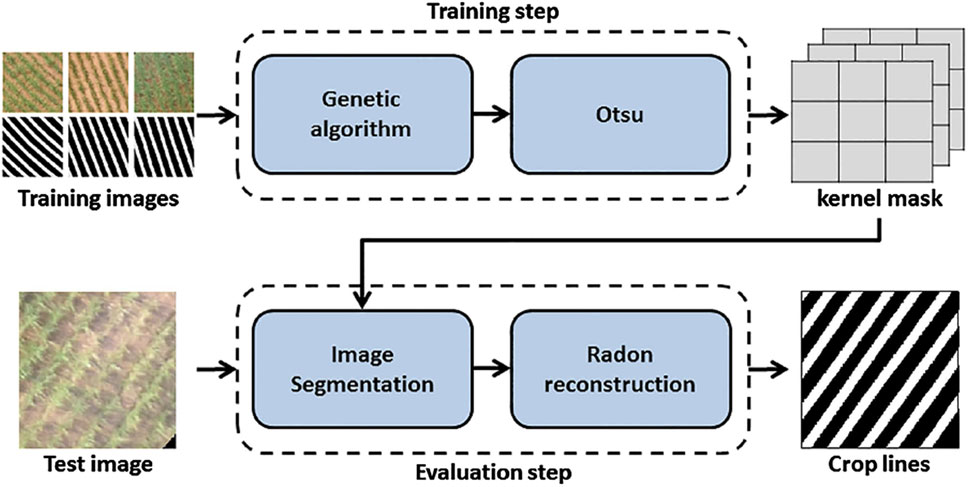
\includegraphics[width=0.6\textheight]{img/2021_Silva_flow_chart.png}
    \caption{Fluxograma do método desenvolvido por  \citeonline{Silva_Escarpinati_Backes_2021}}
    \label{fig:2021_silva_flow_chart}
\end{figure}

Algoritmo Genético (AG) foi utilizado para encontrar uma máscara (\textit{kernel}) (com 27 valores, 9 para cada banda RGB), que é utilizada como filtro convolucional para combinar as bandas da imagem RGB em uma imagem em escala de cinza. O AG foi executado por 2700 gerações, com população de 200 indivíduos e taxa de mutação de 0.05 e \textit{crossover} de 0.8. A função de avaliação (\textit{fitness}) do AG busca maximizar o valor de Coeficiente de \textit{Dice} (comparando a imagem gerada ao aplicar a máscara e em seguida o método de Otsu com a marcação feita pelo especialista).

Para analisar os resultados em função do padrão estocástico do AG e sua convergência, foi utilizado a técnica de validação cruzada com 35 imagens divididas em 5 \textit{fodls}. Os autores afirmam que apesar de ter sido obtido máscaras diferentes para cada cenário, elas foram capazes de produzir uma segmentação semelhante em termos de Coeficiente de \textit{Dice} (CD), sendo assim AG foi capaz de calcular uma mascará eficaz independente de conjunto de treinamento utilizado.

O método Otsu foi avaliado na segmentação (nos 4 \textit{datasets}) utilizando o método global e local. No método local utilizaram janelas (\textit{Window}) de $W \times W$ pixels com deslocamento (\textit{Stride}) $S$ e o operador $OR$ para combinar as binarizações locais em uma única imagem binarizada. O método de Otsu global não obteve bons resultados, provavelmente pela grande extensão dos mosaicos (\textit{datasets}) e a variedade de luminosidade presente neles. Por outro lado o método de Otsu local teve melhores resultados, sendo $W=50$ e $S=25$ obteve um dos melhores resultados. Deste modo, as janelas (valor $W$) menores permitem o método de capturar as características locais com maior precisão, proporcionado uma melhor binarização e consequentemente um Coeficiente de \textit{Dice} mais próximo de 1.

Para detecção das linhas e refinamento depois da binarização foi utilizado a Transformada de Radon com o método de janelamento (\textit{tiling scheme}), utilizando o mesmo esquema usado no método Otsu, com $W$ e $S$. Com melhor resultado com janelas grandes e pequena sobreposição entre as janelas.

Como resultado geral, a detecção das linhas de plantio ficaram próximas do real (marcação do especialista), lidando melhor com linhas retas e não muito bem com linhas curvas, gerando um efeito serrilhamento (\textit{aliasing}) indesejado. 

Na segunda abordagem foi comparado 3 redes neurais artificiais (LinkNet, PSPNet, Unet) na segmentação semântica das linhas de plantio.
O \textRed{encoder} das redes foi substituído pelo da VGG16 pré-treinada a partir do \textit{dataset} ImageNet. Depois foram treinadas por 50 épocas, com taxa de aprendizado de 0.001 utilizando as imagens ($256 \times 256 \times 3$) do primeiro \textit{dataset}.

A LinkNet teve o melhor resultado ($CD = 0.90 \pm 0.0062$), sendo escolhida para testes nos outros \textit{datasets}. O coeficiente de \textit{Dice} foi um pouco pior nos outros \textit{datasets} ($CD >= 0.80$), contudo melhor que a abordagem com AG ($CD <= 0.78$). Também foi analisado a aplicação da transformada de Radon na busca de refinar as linhas no resultado da rede neural, contudo com a aplicação, o CD piorava em muitos casos. Como resultado o CD ficou melhor em algumas imagens e pior em outras, essa é uma parte que ainda precisa ser melhor explorada.

LinkNet teve melhor resultado que o AG por utilizar não apenas o tem avermelhado do solo e esverdado da plantas, mas outras características que as redes neurais conseguem extrair, \textRed{contudo ainda é uma área que merece ser melhor explorada e analisada.} \dotsBlue

\linePage

\citeonline{Oliveira_2020} desenvolveu uma abordagem similar a \citeonline{Silva_2020}, na detecção das linhas de plantio de cana-de-açúcar, utilizando Algoritmo Genético para Multilimiarização, a Transformada
Discreta de Wavelet e Transformada de Hough Probabilística.
\dotsBlue

\linePage

\citeonline{Barbosa_Junior_2021} fez uma análise exploratória do uso de imagens de VANTs na detecção das falhas nas plantações de cana-de-açúcar, variando o GSD (3.5 cm, 6 cm e 8.2 cm), a altura da planta (0.5 m, 0.9 m, 1.2 m e 1.7 m), e o comprimento das falhas (0.5 m, 1.0 m, 1.5 m, 2.0 e 2.5 m). Na identificação das falhas foi utilizado o \textit{software} comercial \textit{Inforow}. Como esperado os melhores resultados foram com GSD pequeno (3.5 cm ou próximo) e plantas com menor altura (e.g., 0.5 m). A altura das plantas foi apontada como um dos fatores mais importantes, seguido pelo GSD, para detecção das falhas nas plantações de cana-de-açúcar. Não sendo possível detectar pequenas falhas  ($<= 1 m$) quando a planta já tinha certa altura ($ >= 1m $) através do \textit{software}. Neste trabalho tem-se sugestões do melhor momento para obter as imagens e sobre o GSD, além de \textRed{mostrar} que mesmo o \textit{software} comercial utilizado não teve bons resultados. \dotsBlue

\linePage

\dotsBlue

\textRed{Fazer uma tabela comparando os trabalhos relacionados?}

Um resumo das principais características e informações dos \textRed{principais} trabalhos relacionados pode ser encontrada na \autoref{tab:trab_rela}.

\begin{landscape}
\begin{table}
\centering
\caption{Comparação entre trabalhos relacionados}
\label{tab:trab_rela}
\begin{tabularx}{\linewidth}{|L|L|L|L|L|L|} 
\hline
\textbf{Trabalho} & \textbf{Cultura} & \textbf{Principais tecnologias} & \textbf{Imagens} & \textbf{Resultado} & \textbf{Lacunas e Limitações} \\ \hline
\cite{Silva_Escarpinati_Backes_2021} & cana-de-açúcar & Algorítimo Genético, Transformada de Radon, Método de Otsu & Imagens de VANTs, com 5.3 cm de GSD e modelo de cor RGB & Detecção das linhas (retas) de plantio próximas do real & Dependência da parte estocástica do AG, não lida bem com linhas curvas e geração de efeito \textit{aliasing} indesejado \\ \hline
cite trab 2 & cultura & principais tecnologias & resolução espacial & resultado & limitações \\ \hline
cite trab 3 & cultura & principais tecnologias & resolução espacial & resultado & limitações \\ \hline
cite trab 4 & cultura & principais tecnologias & resolução espacial & resultado & limitações \\ \hline
cite trab 5 & cultura & principais tecnologias & resolução espacial & resultado & limitações \\ \hline
\end{tabularx}
\end{table}
\end{landscape}

\section{Metodologia de pesquisa}
% => Descreva de forma mais detalhada sua proposta de trabalho, detalhando as estratégias que pretende utilizar para atingir os objetivos propostos. Descreva o método de pesquisa que deverá ser utilizado para validar a sua hipótese incluindo as medidas de avaliação, conjunto de parâmetros, bases de dados e os trabalhos com os quais a sua proposta será comparada.

A metodologia deste projeto é composta por 5 etapas. A primeira etapa é aquisição das imagens/\textit{datsets} coletadas por VANTs utilizando câmera RGB em plantações de cana-de-açúcar. A segunda etapa é o pré-processamento dessas imagens, buscando realçar as linhas de plantio e corrigir pequenas imperfeições.

A terceira etapa é o processamento principal, ou seja, a segmentação das imagens. Onde serão testados e propostos métodos para melhorar a segmentação dessas imagens. Na quarta etapa é feito o prós-processamento para otimizar a segmentação e refinar as linhas detectadas na etapa anterior. Além de tratar linhas incompletas e linhas curvas. Por fim, a avaliação dos resultados da detecção das linhas de plantio.

\subsection{Aquisição das imagens}
\subsection{Pré-processamento}
\subsection{Segmentação}
\subsection{Prós-processamento}
\subsection{Avaliação dos resultados}

\section{Resultados esperados}
% => Liste os resultados mais importantes que você pretende obter a partir de seu trabalho de doutorado.

\textBlue{
1 Um método automático para detecção de linhas de plantio

2 Falhas também?

3 Que consiga lidar bem com linhas retas, linhas curvas, plantações de cana-de-açúcar em vários estágios (idades diferentes) ?

...
}

%\section{Esquema Geral do Texto da Dissertação (opcional)}
% => Descreva o “esqueleto” de sua dissertação, como vai estruturar os capítulos e seções. Dê um título, mesmo que provisório, a sua dissertação.

\section{Cronograma de execução}
% => Detalhe o cronograma das principais etapas de seu trabalho finalizando pela data da defesa.

Para cumprir os objetivos descritos, o plano de pesquisa foi dividido em atividades e seus respectivos meses. O cronograma de atividades do projeto pode ser visualizado na \autoref{tab:cronograma}, onde está definida a
duração das principais atividades.

\begin{table}[htb]
\centering
\caption{Cronograma de atividades}
\label{tab:cronograma}
\begin{tabular}{|c|c|c|c|c|c|c|c|c|c|c|c|c|c|c|c|c|}
\hline
          & \multicolumn{2}{c|}{2021} & \multicolumn{12}{c|}{2022}                    & \multicolumn{2}{c|}{2023} \\ \hline
Atividade & N           & D           & J & F & M & A & M & J & J & A & S & O & N & D & J           & F           \\ \hline
A1        & X           & X           & X & X &   &   &   &   &   &   &   &   &   &   &             &             \\ \hline
A2        &             &             & X & X & X & X &   &   &   &   &   &   &   &   &             &             \\ \hline
A3        &             &             &   &   & X & X & X &   &   &   &   &   &   &   &             &             \\ \hline
A4        &             &             &   &   &   & X & X & X &   &   &   &   &   &   &             &             \\ \hline
A5        &             &             &   &   &   &   & X & X & X &   &   &   &   &   &             &             \\ \hline
A6        &             &             &   &   &   &   &   & X & X & X &   &   &   &   &             &             \\ \hline
A7        &             &             &   &   &   &   &   &   & X & X &   &   &   &   &             &             \\ \hline
A8        &             &             &   &   &   &   &   &   &   & X & X & X &   &   &             &             \\ \hline
A9        &             &             &   &   &   &   &   &   &   &   &   & X & X & X & X           &             \\ \hline
A10       &             &             &   &   &   &   &   &   &   &   &   &   &   &   & X           & X           \\ \hline
\end{tabular}
\end{table}

As atividades são descritas abaixo:

\begin{itemize}
    \item A1: revisão bibliográfica sobre os métodos de segmentação e detecção de linhas de plantio.
    \item A2: estudo dos algoritmos e métodos encontrados na literatura correlata sobre segmentação de imagens.
    \item A3: estudo dos algoritmos e métodos encontrados na literatura correlata sobre \textit{deep learning} na segmentação de imagens.
    \item A4. Avaliação dos algoritmos estudados com relação a possibilidade de aplicar as técnicas estudadas no contexto do nosso trabalho.
    \item A5: aplicação e análise dos algoritmos e métodos encontrados em imagens reais.
    \item A6: avaliação dos resultados e propostas de melhorias.
    \item A7: readequação dos parâmetros e mais experimentos (caso necessário).
    \item A8: elaboração e submissão de artigos científicos para periódicos e/ou congresso da área.
    \item A9: elaboração da dissertação (escrita e preparação para a defesa).
    \item A10: defesa da dissertação.
\end{itemize}

% \section{Justificativa pelo atraso na entrega do projeto (tópico obrigatório somente no caso de entrega do projeto foram do prazo regulamentar*)}
% => Descrever as justificativas que levaram ao atraso na entrega do projeto.

% \textbf{*RI-PPGCO/UFU, art. 18, parágrafo único:
% O projeto de Dissertação de Mestrado deverá ser apresentado pelo estudante até o final do segundo semestre letivo, contado a partir da matrícula de ingresso como aluno regular.}

\bigskip
\noindent \boxYellow{Uberlândia, 10 de novembro de 2021.}
% Encaminhar para o e-mail cpgfacom@ufu.br

% \section{Bibliografia}
\bibliography{references}

\end{document}
